\section{\textcolor[HTML]{D32F2F}{Videreutvikling av produktet}}
\label{videre}

I brukertestene gruppen gjorde med wireframe-prototypen fungerte det aller meste veldig bra. Noen endringer var det likevel aktuelt å gjøre dersom det skulle vært jobbet videre med produktet. En av disse endringene ville være å velge om appen skal ha knapper eller menylinje på startsiden. I Axure-modellen var det både knapper for navigasjon og en menylinje i bunn med de samme ikonene. Dette gjorde testpersonene noe forvirret, og kan godt sies å være unødvendig. Gruppen gjorde seg opp noen tanker rundt dette. Her kunne man ha tatt bort knappene, og beholdt knappen for å opprette ny ønskeliste. Menylinjen i bunn ville vært den samme, og åpningstider eller annen informasjon fra senteret kunne fått mer fokus. For eksempel nyheter eller tilbud hos butikkene.

%Hvorfor produktet vårt er et bra konsept, hvem vil få noe ut av dette?\\ (kundenes fordeler og butikkenes fordeler og sirkus shopping sine fordeler)

\subsection{Fra kundens perspektiv}
Gjennom prosessen har gruppen hatt en dialog med brukerne av sluttproduktet. Det har blitt gjennomført både intervjuer, spørreundersøkelse og tester. Dette har gitt gruppen informasjon om hva brukerne har behov for og hva de savner i sin handleopplevelse. Gruppen fikk flere tilbakemeldinger om at løsningen som ble presentert var attraktiv og spennende. Flere av testpersonene så flere fordeler ved å benytte seg av en slik app, og ved å kunne handle på kjøpesentre som er strukturert på en annen måte enn de tradisjonelle kjøpesentrene. Hovedargumentene som brukerne nevnte var tidsbesparelse, enkelt å handle inn til andre (julegaver, fødselsdagspresanger ol.), og at det vil bli litt som en nettshopping bare at man får varene med en gang. Dette var det flere som syntes var positivt.
\\\\
Det var også flere som nevnte at de ikke så for seg at de kom til å bruke det. Argumentet her var at dersom man kun skal ha én ting, vil det være mer effektivt og tidsbesparende å gå inn i butikken og kjøpe varen i kassen uten å måtte gå gjennom prosessen med appen. Av dette forstod gruppen at målgruppen for produktet ikke bare er kjønn, alder eller livssituasjon. Målgruppen må også spesifiseres inn på formålet med handleturen. Gruppen reflekterte tidlig i prosessen over det at kunder på et senter gjerne er på en større handletur, og har bedre tid enn en kunde som kun skal raskt innom en jernvarehandel for å kjøpe en mutter. Det så vi igjen senere. Målet for produktet vil altså være de kundene som er på en større handletur, og er på senteret for å handle. I det menes at de har tid, er ute etter å kikke etter produkter og åpen for nye impulser. Kundene som kun skal ha en vare og utfører hele handleturen på fem minutter er ikke målet for appen.

\subsection{Fra kjøpesenterets perspektiv}
Gruppen har også vært i kontakt med ansatte i butikker på Sirkus shopping i løpet av prosessen. Gruppen presenterte ideen for de ansatte, og responsen var stort sett positiv. De ansatte uttrykte at å kun ha noen eksemplarer av hver vare vil lette arbeidet. Dersom det kun finnes to jakker i hver størrelse av en modell ute i butikken, vil det være langt lettere for de ansatte å holde orden i butikken. I dag har butikkene ofte titalls eksemplarer av hver størrelse ute i butikken, og ettersom kundene leter gjennom produktene må de ansatte brette og rydde opp slik at butikken er ryddig til enhver tid. En annen ting som ble poengtert var at et samlet lager vil redusere behovet for å fylle på varer i butikk, samt redusere antall varer som må selges med rabatt pga. flekker eller andre ting som skjer med produkter på utstilling.
\\\\
De ansatte gruppen snakket om nevnte ingen ting om at det ville være negativt å ta i bruk en modell som dette, men gjennom tilbakemeldinger i undervisningen (både fra forelesere og medstudenter) ble vi gjort oppmerksomme på noen ulemper. En utfordring kan oppstå med tanke på sysselsetting. Gruppen så for seg et lager der alt plukkes automatisk av roboter, slik det gjøres på lagrene til nettbutikker som f.eks. Komplett.no. Som vist i Figur \ref{fig:lager} stables kasser hvor det så er små roboter som plasserer varene kunden har bestilt i kassen. Alt går automatisk, og man trenger ikke ansette egne personer til å bemanne lageret. Noen må selvfølgelig fylle på varer når de kommer med leveranser, men bemanningsbehovet er langt lavere enn ved et lager bemannet av kun mennesker. Noen stilte dermed et spørsmål om hva dette vil gjøre. For kjøpesenteret/butikkene vil dette gjøre at lønnsutgiftene blir lavere, men det vil også koste mye penger å kjøpe inn et slikt system.

\begin{figure}[H]
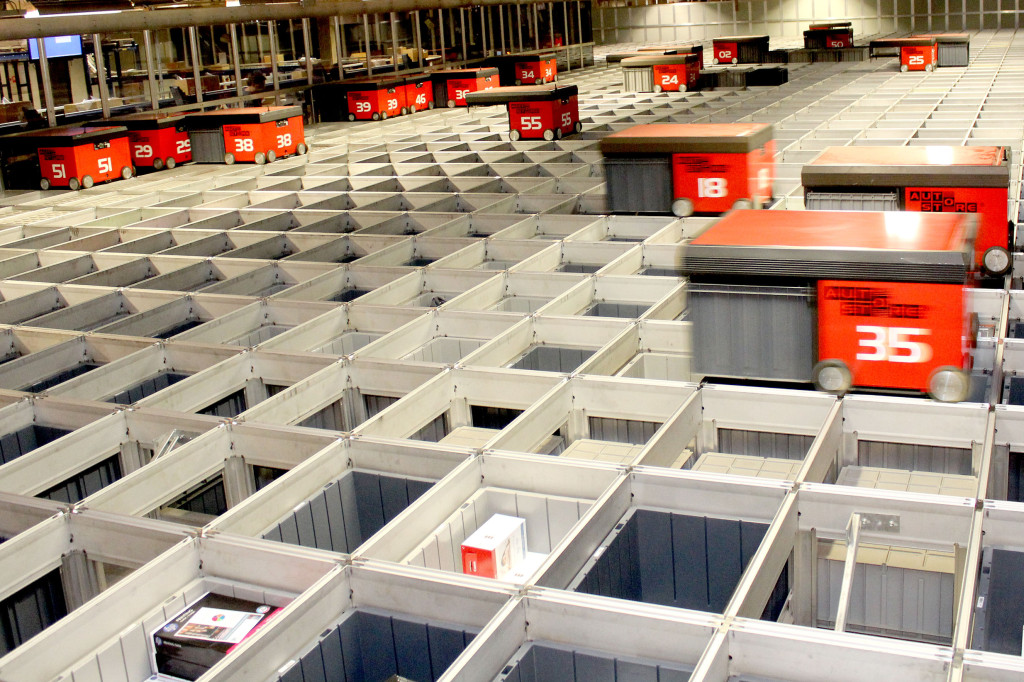
\includegraphics[scale=0.4]{images/lager}
\centering %centering the image
\caption{Lager hos Komplett.no\cite{komplett}}
\label{fig:lager}
\end{figure}

\noindent Alternativet til å kjøpe inn et robotsystem for lageret er at ansatte plukker varene. Dette er muligens det mest realistiske i første omgang for kjøpesenteret. Med denne modellen vil mange av de som i dag jobber i kassen flyttes over til lageret, og heller jobbe med å pakke varer. Det betyr ikke at alle ansatte i butikkene vil forsvinne, for det vil fortsatt være behov for veiledning i butikken. Kundene har ofte spørsmål om varenes egenskaper, forskjeller mellom produkter og tips til kjøp. Dette behovet vil fortsatt eksistere selv om man bytter ut handlevognen med en applikasjon og omstrukturerer butikkene.
\\\\
Et annet poeng som ble trukket fram er at appen viser en totalsum for handlevognen. Dette er gunstig for kunden, som da kan se hvor mye hun har i kurven. Da har kunden kontroll på pris og hvor mye det koster, likt man har i nettbutikker. Dette kan være noe butikkene ikke setter stor pris på, siden kunden med ett blir mer observant på hva totalprisen er. Det blir dermed antakeligvis vanskeligere å drive med mersalg, siden kunden er bevisst på kjøpesummen. 

%Kvalitetskriterier: styrke av appen vs. nytte av appen vs. service den gir

%Evaluer opp mot 
%- Brukersentrert metode (forelsening)
%- kvalitetskristerier ((forelesning)
%- kroppsnær teknologi (forelesning)
%- Kvalitativ metode og analyse (forelesning)




